\documentclass[11pt]{article}

\usepackage{hyphenat}
\usepackage{xspace}
\usepackage{amsmath}
\usepackage{graphicx}
\usepackage{subfigure}
\usepackage{wrapfig}
\usepackage{fancyhdr}
\usepackage{hyperref}
\usepackage{boxedminipage}
\usepackage{color}
\usepackage{helvet}
\usepackage[utf8]{inputenc}
\usepackage{natbib}
\usepackage{todonotes}
\usepackage{blindtext}

\setlength{\bibsep}{0.0pt}

%%%%%%%%%%%%%%%%%%%%%%%%%%%%%%%%%%%%%%%%%%%%%%%%%%%%%%%%%%%%
\newcommand{\ThesisTitle}{The Impact of Conventional Commits on Software Project Quality\xspace}
\newcommand{\ProjectAcronym}{\textsc{ICCSPQ}\xspace}

% % some commands for commenting
\usepackage{ifthen}
\usepackage{amssymb}
\usepackage[normalem]{ulem} % for \sout
\newboolean{showcomments}
\setboolean{showcomments}{true} % toggle to show or hide comments
\ifthenelse{\boolean{showcomments}}
  {
		%\usepackage{showkeys} %Show lables and refs
		\newcommand{\nbb}[2]{
		% \fbox{\bfseries\sffamily\scriptsize#1}
		\fcolorbox{black}{yellow}{\bfseries\sffamily\scriptsize#1}
		{\sf$\blacktriangleright$\textcolor{blue}{\textit{#2}}$\blacktriangleleft$}
		% \marginpar{\fbox{\bfseries\sffamily#1}}
		}
		
		\newcommand{\version}{\emph{\scriptsize$-$9.2.2011$-$}}
		\newcommand{\remarks}[1]{\color{red}[#1]\color{black}}
		\newcommand{\copied}[1]{\color{green}[#1]\color{black}}
		\newcommand{\modified}[1]{\color{blue}[#1]\color{black}}
		\newcommand{\raw}{$\rightarrow$}
		\newcommand{\old}[1]{\textcolor[rgb]{0.8,0.8,0.8}{#1}}%old stuff
		\newcommand{\ins}[1]{\textcolor{blue}{\uline{#1}}} % please insert
		\newcommand{\del}[1]{\textcolor{red}{\sout{#1}}} % please delete
		\newcommand{\chg}[2]{\textcolor{red}{\sout{#1}}{\raw}\textcolor{blue}{\uline{#2}}} % please change
		\newcommand{\ugh}[1]{\textcolor{red}{\uwave{#1}}} % please rephrase
  }
  {
		\newcommand{\nbb}[2]{}
		\newcommand{\remarks}[1]{}
		\newcommand{\modified}[1]{#1}
		\newcommand{\copied}[1]{#1}
		\newcommand{\version}{}
		\newcommand{\old}[1]{#1} % please rephrase
		\newcommand{\ugh}[1]{#1} % please rephrase
		\newcommand{\ins}[1]{#1} % please insert
		\newcommand{\del}[1]{} % please delete
		\newcommand{\chg}[2]{#2} % please change
  }
% reviewer and advisor comments
\newcommand{\lars}[1]{\nbb{Lars}{#1}}
\newcommand{\avh}[1]{\nbb{Andre}{#1}}
\newcommand{\dusan}[1]{\nbb{Dusan}{#1}}

% if you want to add a TODO
\newcommand{\TODO}[1]{\todo[inline]{#1}}

\newenvironment{compact_itemize}{

 \begin{itemize}
  \setlength{\itemsep}{1pt}
  \setlength{\parskip}{0pt}
  \setlength{\parsep}{0pt}
}{
  \end{itemize}
 }

% Dealing with identifiers
\newcommand{\mathid}[1]{\textit{#1}}
\newcommand{\codeid}[1]{\texttt{#1}}
% \let\codeid=\mathid
\def\|#1|{\mathid{#1}}
\def\<#1>{\codeid{#1}}


%%%%%%%%%%%%%%%%%%%%%%%%%%%%%%%%%%%%%%%%%%%%%%%%%%%%%%%%%%%%

\renewcommand{\familydefault}{\sfdefault}

\voffset-0.0cm
\hoffset0.0cm
\topmargin0.0cm
\headheight0.0cm
\headsep0.0cm
\topskip0.0cm
\textwidth 16cm
\textheight 22cm
\oddsidemargin-0.245cm
\evensidemargin-0.245cm
\footskip1.0cm

%%%%%%%%%%%%%%%%%%%%%%%%%%%%%%%%%%%%%%%%%%%%%%%%%%%%%%%%%%%%
%Header +Footer
%%%%%%%%%%%%%%%%%%%%%%%%%%%%%%%%%%%%%%%%%%%%%%%%%%%%%%%%%%%%

\pagestyle{fancyplain}
\usepackage{lastpage}
\fancyhf{}
\renewcommand{\headrulewidth}{0pt} % remove lines
\renewcommand{\footrulewidth}{0.5pt}
\lfoot{ \fancyplain{}{\ThesisTitle} }
\rfoot{ \fancyplain{}{Page \thepage \xspace of \pageref{LastPage}} }
%%%%%%%%%%%%%%%%%%%%%%%%%%%%%%%%%%%%%%%%%%%%%%%%%%%%%%%%%%%%
%\usepackage{multibib}
%\newcites{own}{   }


%%%%%%%%%%%%%%%%%%%%%%%%%%%%%%%%%%%%%%%%%%%%%%%%%%%%%%%%%%%%
% Summaries and results
%%%%%%%%%%%%%%%%%%%%%%%%%%%%%%%%%%%%%%%%%%%%%%%%%%%%%%%%%%%%

\newenvironment{keypoints}{%
\medskip\noindent
\begin{boxedminipage}{\linewidth}\vspace{6pt}
\begin{compact_itemize}}{%
\end{compact_itemize}\vspace{-6pt}
\end{boxedminipage}}


%%%%%%%%%%%%%%%%%%%%%%%%%%%%%%%%%%%%%%%%%%%%%%%%%%%%%%%%%%%%
% Document start
%%%%%%%%%%%%%%%%%%%%%%%%%%%%%%%%%%%%%%%%%%%%%%%%%%%%%%%%%%%%

\begin{document}

\section*{\ThesisTitle\ -- (\ProjectAcronym)}
\subsection*{---\,Proposal for a Bachelor's Thesis\,---}

\sloppy

\noindent Anna Freidl

\noindent Advised by: Alexander Schultheiß

\begin{center}
\line(1,0){450}
\end{center}

\section*{Topic Description}
Conventional Commits is a lightweight convention for structuring commit messages. \cite{conventionalcommits} It provides a standardized format for describing the nature of changes made to a codebase, making it easier for developers to understand and navigate the project's history. This proposal outlines a potential research study to investigate the impact of Conventional Commits on software project quality.

\paragraph{Motivierende Arbeiten:} 
\begin{itemize}
\item \cite{refrecommendation} Traditionelle Ansätze zur Verbesserung der Softwarequalität ("Refactoring") basieren auf der Analyse des Codes. Diese identifizieren zwar Verbesserungsmöglichkeiten, berücksichtigen aber nicht immer den aktuellen Kontext des Entwicklers. Entwickler dokumentieren zwar manchmal ihre Refactoring-Absichten in Commit-Nachrichten, können dabei aber relevante Verbesserungen übersehen. Diese Studie zeigt, dass die Analyse von Commit-Nachrichten zur Identifikation von Refactoring-Möglichkeiten eingesetzt werden kann und bessere Ergebnisse liefert als die Codeanalyse allein.

\item \cite{commitanalysis} Diese Studie untersucht den Zusammenhang zwischen Emotionen in Commit-Nachrichten und verschiedenen Faktoren in Open-Source-Projekten. Man analysiert die Gefühlsrichtung der Kommentare mithilfe eines Werkzeugs ("lexical sentiment analysis"). Die Ergebnisse zeigen, dass z.B. Java-Projekte negativere Kommentare aufweisen und verteilt arbeitende Teams positiver kommunizieren. Montags herrscht anscheinend die schlechte Laune, denn die Commit-Nachrichten fallen negativer aus. Die Studie benötigt zwar eine größere Datenbasis, bietet aber interessante Einblicke in die Gefühlswelt von Entwicklern.
\end{itemize}

\section{State of the art and preliminary work}

\subsection{The first group of approaches} 
\subsection{The second group of approaches} \label{subsec_SecondGroupRelated}

\section{Objectives and work program}

\subsection{Anticipated total duration of the project}

\subsection{Objectives}

%short introduction of work package macros (for consistency)
\newcommand{\WPone}{Something, something and doing something}
\newcommand{\WPtwo}{Working in a coal mine}
\newcommand{\WPthree}{Sixteen tons}
\newcommand{\WPfour}{Celebration preparation}

\subsection{Work programme incl. proposed research methods}
\label{subsec-workprogram}

\begin{figure}[ht]
\centering
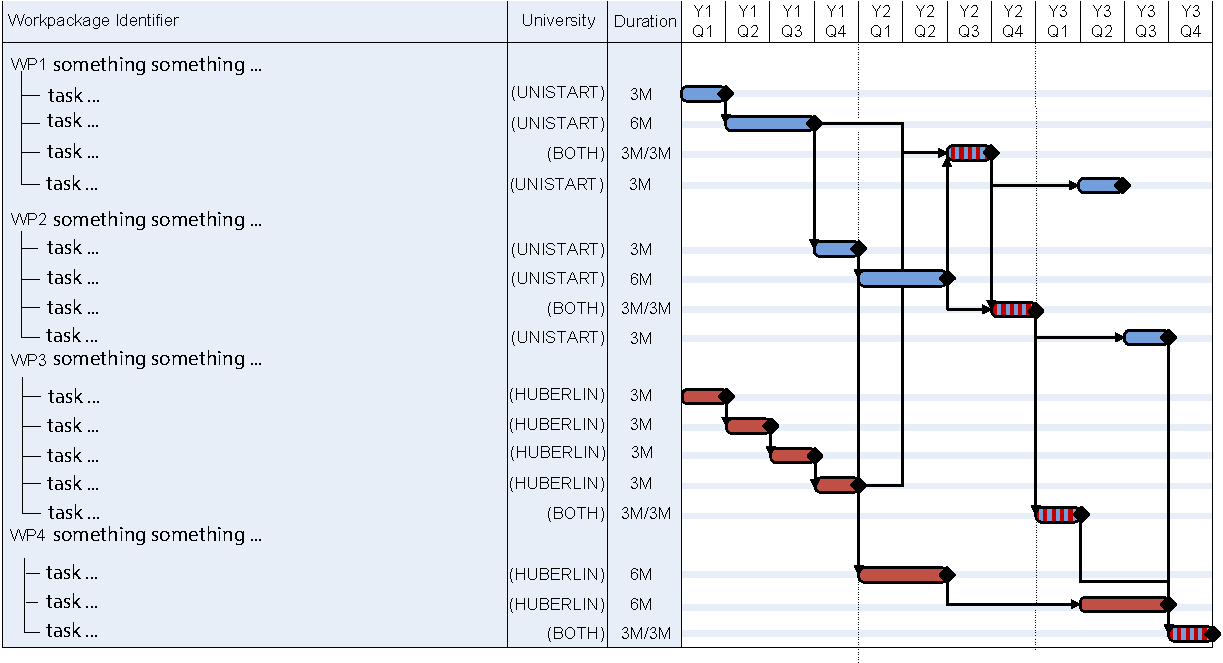
\includegraphics[width=\linewidth]{img/gantt}
\caption{An example work plan of another project}
\label{fig:work-plan}
\end{figure}


% In this section, subsections are organized by packages -- AZ
\newcounter{wp}
\let\oldthesubsection=\thesubsection
\def\thesubsection{WP\arabic{wp}}
% \def\package#1{\subsection[\protect\thesubsection{} {#1}]{#1}}
\def\package#1{\addtocounter{wp}{1}\subsection{#1}}

% Use \task to introduce tasks
\let\oldthesubsubsection=\thesubsubsection
\def\thesubsubsection{\thesubsection.\arabic{subsubsection}}
% \def\task#1{\subsubsection[\thesubsubsection{} {#1}]{#1}}
\let\task=\subsubsection

\package{\WPone.}
\label{wp:something}

\paragraph{Challenges and motivation.}

\paragraph{Research plan and individual research tasks.}

\task{Refining something}
\label{task-wp1-1}

\paragraph{Research methodology and validation strategy.}

\task{The second important task}
\label{task-wp1-2}

%%%%%%%%%%%%%%%%%%%% New WP Starts
\package{\WPtwo.}
\label{wp:work-something}

%%%%%%%%%%%%%%%%%%%% New WP Starts
\package{\WPthree.}
\label{wp:do-this}

%%%%%%%%%%%%%%%%%%%% New WP Starts
\package{\WPfour.}
\label{wp:do-that}


\let\thesubsection=\oldthesubsection
\let\thesubsubsection=\oldthesubsubsection
\setcounter{subsection}{3}

\subsection{Data handling}
\subsection{Other information}

\section{Bibliography}

\bibliographystyle{alpha}
\bibliography{bibliography}

\section{Project requirements}
\subsection{Cooperation with other researchers}
\subsection{Scientific equipment}

\subsection{Project-relevant interests in commercial enterprises}

\end{document}

